\documentclass[tikz,border=8pt]{standalone}
\usepackage{amsmath,amssymb}
\usetikzlibrary{arrows.meta,calc,decorations.markings,decorations.pathmorphing,patterns,shapes.geometric,positioning}

\begin{document}
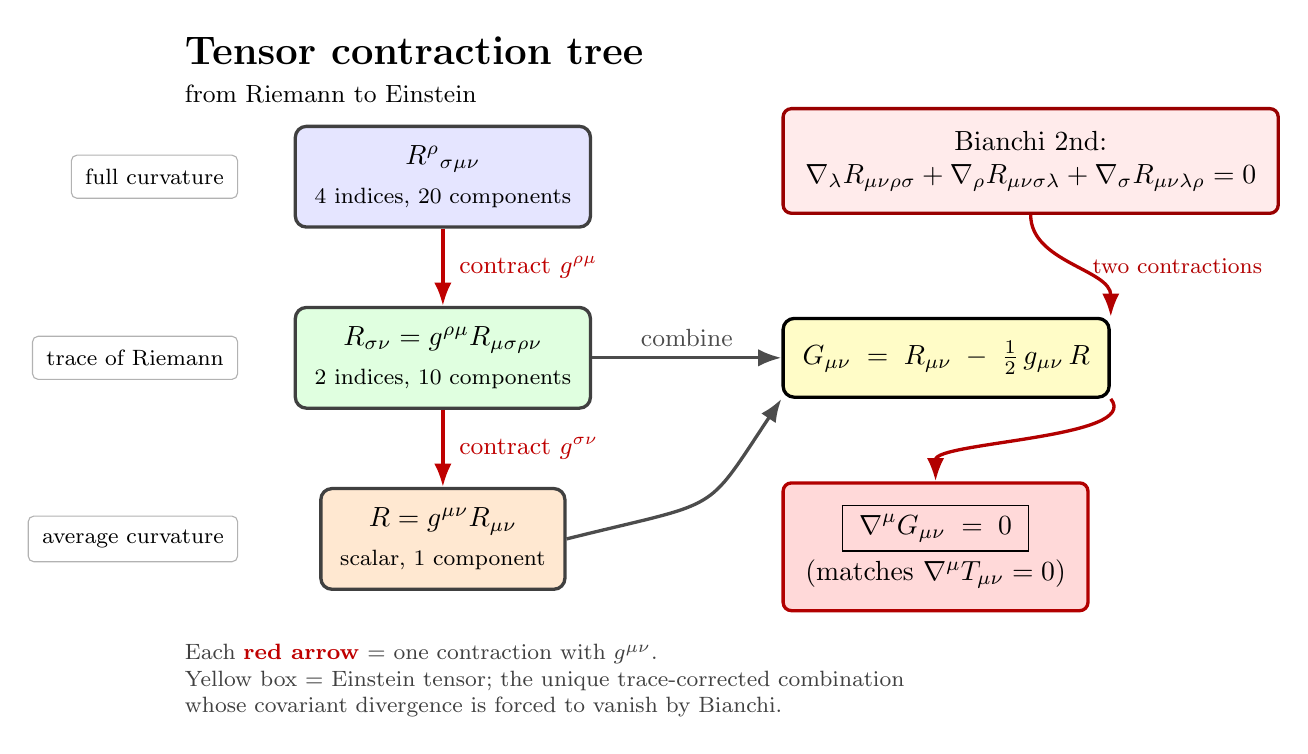
\begin{tikzpicture}[>=Latex,
  tnode/.style={rectangle, rounded corners=4pt, draw=black!75, very thick,
                inner sep=7pt, font=\normalsize, align=center, minimum height=1.0cm},
  riemannN/.style={tnode, fill=blue!10},
  ricciN/.style={tnode, fill=green!12},
  scalarN/.style={tnode, fill=orange!18},
  einsteinN/.style={tnode, fill=yellow!22, draw=black, very thick, minimum width=4.0cm},
  bianchiN/.style={rectangle, draw=red!60!black, very thick, rounded corners=3pt,
                   fill=red!8, inner sep=8pt, font=\normalsize, align=center},
  contract/.style={->, very thick, red!75!black},
  combine/.style={->, very thick, black!70},
  faintbox/.style={rectangle, rounded corners=2pt, draw=black!30,
                   inner sep=5pt, font=\footnotesize, align=center, fill=white}]

  % --- Title ---------------------------------------------------------------
  \node[font=\Large\bfseries, anchor=west] at (-3.4, 6.6) {Tensor contraction tree};
  \node[font=\small, anchor=west] at (-3.4, 6.05) {from Riemann to Einstein};

  % --- Top: Riemann tensor (4 indices) -------------------------------------
  \node[riemannN] (Riem) at (0, 5.0) {$R^{\rho}{}_{\sigma\mu\nu}$ \\[2pt] {\footnotesize 4 indices, 20 components}};

  % --- Middle: Ricci tensor (2 indices) ------------------------------------
  \node[ricciN] (Ric) at (0, 2.7) {$R_{\sigma\nu}=g^{\rho\mu}R_{\mu\sigma\rho\nu}$ \\[2pt] {\footnotesize 2 indices, 10 components}};

  % --- Bottom: Ricci scalar (0 indices) ------------------------------------
  \node[scalarN] (Rsc) at (0, 0.4) {$R = g^{\mu\nu} R_{\mu\nu}$ \\[2pt] {\footnotesize scalar, 1 component}};

  % --- Arrows from Riemann to Ricci to R -----------------------------------
  \draw[contract] (Riem) -- node[right, font=\small, red!75!black, xshift=2pt]
        {contract $g^{\rho\mu}$} (Ric);
  \draw[contract] (Ric) -- node[right, font=\small, red!75!black, xshift=2pt]
        {contract $g^{\sigma\nu}$} (Rsc);

  % Side label: information lost at each step
  \node[faintbox, anchor=east] at (-2.6, 5.0) {full curvature};
  \node[faintbox, anchor=east] at (-2.6, 2.7) {trace of Riemann};
  \node[faintbox, anchor=east] at (-2.6, 0.4) {average curvature};

  % --- Right side: Einstein tensor box -------------------------------------
  \node[einsteinN, anchor=west] (Ein) at (4.3, 2.7)
    {$G_{\mu\nu} \;=\; R_{\mu\nu} \;-\; \tfrac{1}{2}\,g_{\mu\nu}\,R$};

  % Arrow from Ricci to Einstein
  \draw[combine] (Ric.east) -- node[above, font=\small]{combine} (Ein.west);

  % Arrow from R into Einstein box (curved)
  \draw[combine] (Rsc.east) .. controls +(2.0, 0.5) and +(-1.0, -1.5) .. (Ein.south west);

  % --- Bianchi identity box ------------------------------------------------
  \node[bianchiN, anchor=west] (Bi) at (4.3, 5.2)
    {Bianchi 2nd: \\
     $\nabla_\lambda R_{\mu\nu\rho\sigma} + \nabla_\rho R_{\mu\nu\sigma\lambda} + \nabla_\sigma R_{\mu\nu\lambda\rho} = 0$};

  % --- Conservation arrow (the key result) ---------------------------------
  \node[bianchiN, fill=red!15, draw=red!70!black, anchor=west] (Cons) at (4.3, 0.3)
    {$\boxed{\;\nabla^{\mu} G_{\mu\nu} \;=\; 0\;}$ \\[2pt] (matches $\nabla^\mu T_{\mu\nu}=0$)};

  % Arrow from Bianchi to conservation
  \draw[->, very thick, red!70!black] (Bi.south) .. controls +(0, -0.6) and +(0, 0.6) ..
       node[right, font=\footnotesize, red!70!black, xshift=4pt]
       {two contractions} (Ein.north east);
  \draw[->, very thick, red!70!black] (Ein.south east) .. controls +(0.4, -0.5) and +(0, 0.5) .. (Cons.north);

  % --- Bottom legend / contractor key --------------------------------------
  \node[font=\footnotesize, anchor=west, align=left, text=black!75]
    at (-3.4, -1.4)
    {Each {\color{red!75!black}\textbf{red arrow}} = one contraction with $g^{\mu\nu}$.\\
     Yellow box = Einstein tensor; the unique trace-corrected combination\\
     whose covariant divergence is forced to vanish by Bianchi.};

\end{tikzpicture}
\end{document}
